\documentclass[twoside, a4paper, 10pt]{report}
\usepackage[italian]{babel}
\usepackage[utf8]{inputenc}
\usepackage[margin=1in]{geometry}
\usepackage{graphicx}
\usepackage{fancyhdr}
\usepackage{array}
\usepackage{colortbl}
\usepackage{lastpage}
\usepackage{titlesec}
\usepackage{float}
\usepackage{subcaption}
\usepackage{hyperref}
\usepackage{afterpage}

% Ridefinizione per il titolo dei capitoli
\titleformat{\chapter}[hang]{\LARGE\bfseries}{\thechapter}{1em}{} 
\titlespacing{\chapter}{0pt}{0pt}{1em}

% Definizione della path per le immagini
\graphicspath{{../images/}}

% Set the version of the document
\newcommand{\version}{1.0} 
\newcommand{\ProjectTitle}{SatisTrento}
\newcommand{\ProjectTitleShort}{satisTrento}
\newcommand{\FileName}{D1-\ProjectTitleShort-descrizioneProgetto}

% Definizione dei dati del documento
\title{Descrizione di Progetto - \ProjectTitle}
\author{Facchini Luca, Prigione Luca, Faa Enrico}
\date{A.A. 2024/2025}

% Definizione metadati PDF
\hypersetup{
    pdftitle={\ProjectTitle},
    pdfauthor={Facchini Luca, Prigione Luca, Faa Enrico},
    pdfsubject={Descrizione di Progetto},
    pdfkeywords={\ProjectTitle, Descrizione di Progetto, Documento di Analisi, Comune di Trento, UniTN}
}

% Definizione counter Requisiti Funzionali
\newcounter{rfCounter}
\newcounter{rnfCounter}

% Definisci un nuovo comando per il formato RF/RNF
\newcommand{\RF}{RF\arabic{rfCounter}}
\newcommand{\RNF}{RNF\arabic{rnfCounter}}

% Definizione nuovo comando per lista con RF/RNF automatici in modo che NON si resettino ad ogni lista
% Ambiente per la lista di RF
\newenvironment{rfList}{
    \begin{list}{\textbf{\RF:}}{ \setlength{\itemsep}{0pt} } % Lista RF
        \setcounter{rfCounter}{\value{rfCounter}} % Mantieni il valore corrente
}{\end{list}}

% Ambiente per la lista di RNF
\newenvironment{rnfList}{
    \begin{list}{\textbf{\RNF:}}{ \setlength{\itemsep}{0pt} } % Lista RNF
        \setcounter{rnfCounter}{\value{rnfCounter}} % Mantieni il valore corrente
}{\end{list}}

% comandi per gli item delle liste RF e RNF
\newcommand{\rfItem}{\stepcounter{rfCounter}\item}
\newcommand{\rnfItem}{\stepcounter{rnfCounter}\item}

% Rimozione scritta "Capitolo" dai titoli dei capitoli
\renewcommand{\chaptermark}[1]{%
    \markboth{
        \thechapter.\ #1%
    }{}%
}
% Definizione del layout della pagina
\fancypagestyle{stdPage}{
    \setlength{\headheight}{24.0pt} 
    \renewcommand{\footrulewidth}{0.4pt}
    \fancyhead{}
    \fancyfoot{}
    \fancyhead[LE,RO]{\begin{tabular}{l l}
        \textbf{Document:} & Descrizione di progetto \\
        \textbf{Version:} & \version
    \end{tabular}}
    \fancyfoot[LE,RO]{\thepage / \pageref*{LastPage}}
    \fancyhead[LO,RE]{\leftmark}
}
\fancypagestyle{plain}{
    \pagestyle{stdPage}
}
\fancypagestyle{index}{
    \pagestyle{stdPage}
    \fancyfoot[LE,RO]{\thepage}
}

\fancypagestyle{emptyPage}{
    \setlength{\headheight}{24.0pt} 
    \renewcommand{\headrulewidth}{0pt}
    \fancyhead{}
    \fancyfoot{}
}

% Definizione della pagina bianca
\newcommand\blankpage{%
    \null
    \thispagestyle{empty}%
    \newpage}

\begin{document}
    \pagestyle{fancy}
    \pagenumbering{Roman} 
    
    \begin{titlepage}
        \thispagestyle{emptyPage}
        
\includegraphics[width=0.33\textwidth]{logoUni.png}
        \vspace{1cm}\newline
        \textbf{Progetto:}
        \vspace{0.5cm}
        \begin{center}
            \textbf{\Huge{\ProjectTitle}}
        \end{center}
        \vspace{1cm}
        \textbf{Titolo del documento:}
        \vspace{0.5cm}
        \begin{center}
            \textbf{\huge{Descrizione di Progetto}}
        \end{center}
        \vspace{1cm}
        \textbf{Document Info}
        \vspace{0.5cm}
        % Table with document info
        \begin{center}
            \begin{tabular}{|l|l|l|c|}  
                \hline
                {\cellcolor[rgb]{0,0.502,1}}\textcolor{white}{\textbf{Doc. Name}}   & \FileName & {\cellcolor[rgb]{0,0.502,1}}\begin{tabular}[c]{@{}>{\cellcolor[rgb]{0,0.502,1}}l@{}}\textcolor{white}{\textbf{Doc.}}\\\textcolor{white}{\textbf{Number}}\end{tabular} & D1 V\version  \\ 
                \hline
                {\cellcolor[rgb]{0,0.502,1}}\textcolor{white}{\textbf{Description}} & \multicolumn{3}{l|}{Documento di analisi dei requisiti funzionali, non funzionali e front-end}                                                                                                                               \\
                \hline
            \end{tabular}
        \end{center}
        % Document authors (1 per line) with name and ID aligned to the right but with some space from the right border 
        \vspace{1.5in}
        \vfill
        \begin{flushright}
            \rightskip=2cm
            \begin{tabular}{r l}
                \multicolumn{2}{c}{\textbf{Authors}} \\
                Facchini Luca & 245965 \\
                Prigione Luca & 242880 \\
                Faa Enrico & 243889
            \end{tabular}
        \end{flushright}
        \vfill
    \end{titlepage}
    % \afterpage{\blankpage} % Uncomment this line if to print as a booklet
    \begingroup
        \setcounter{tocdepth}{0}
        \tableofcontents
        \thispagestyle{index}
    \endgroup
    \pagestyle{stdPage}
    % \afterpage{\blankpage} % Uncomment this line if to print as a booklet
    \newpage
    \pagenumbering{arabic} 
    
    \chapter{Il progetto \ProjectTitle}
% Grid with 1 row and 3 columns for images inside the folder slides
\begin{figure}[H]
    \begin{subfigure}{0.33\textwidth}
        
\includegraphics[width=\textwidth]{slides/Diapositiva2.PNG}
        \caption{I problemi}
    \end{subfigure}
    \begin{subfigure}{0.33\textwidth}
        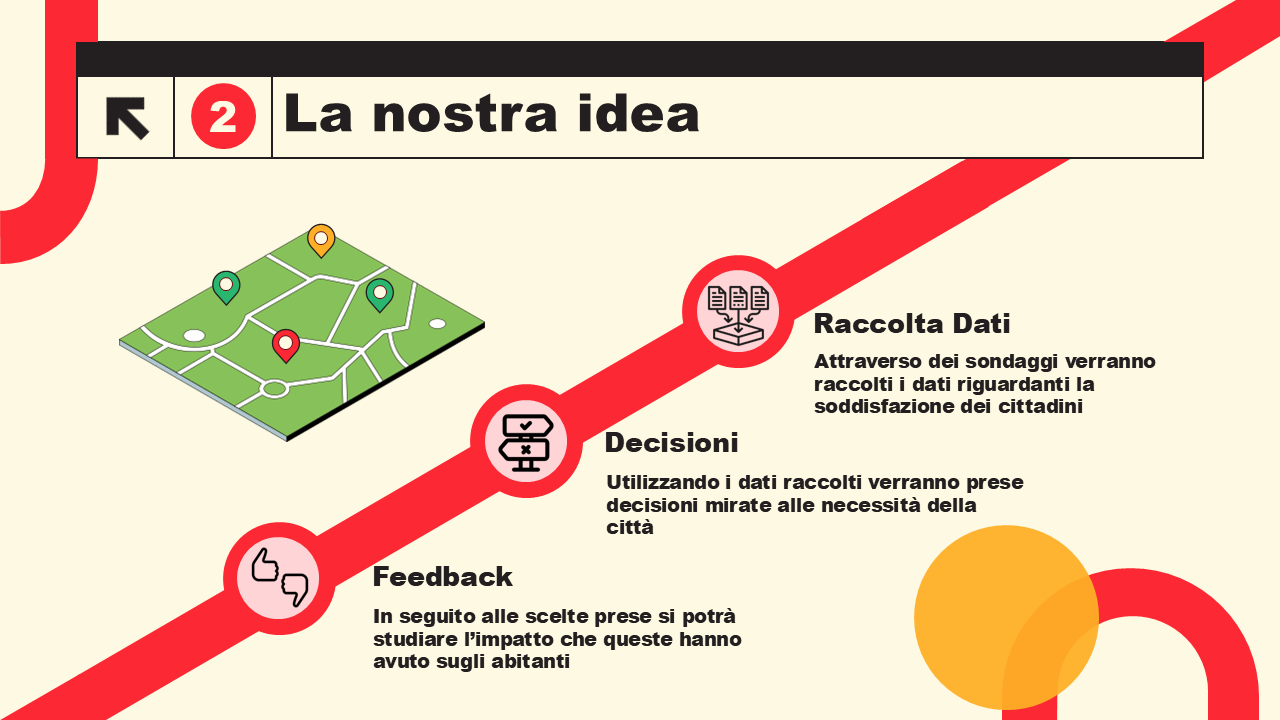
\includegraphics[width=\textwidth]{slides/Diapositiva3.PNG}
        \caption{La soluzione}
    \end{subfigure}
    \begin{subfigure}{0.33\textwidth}
        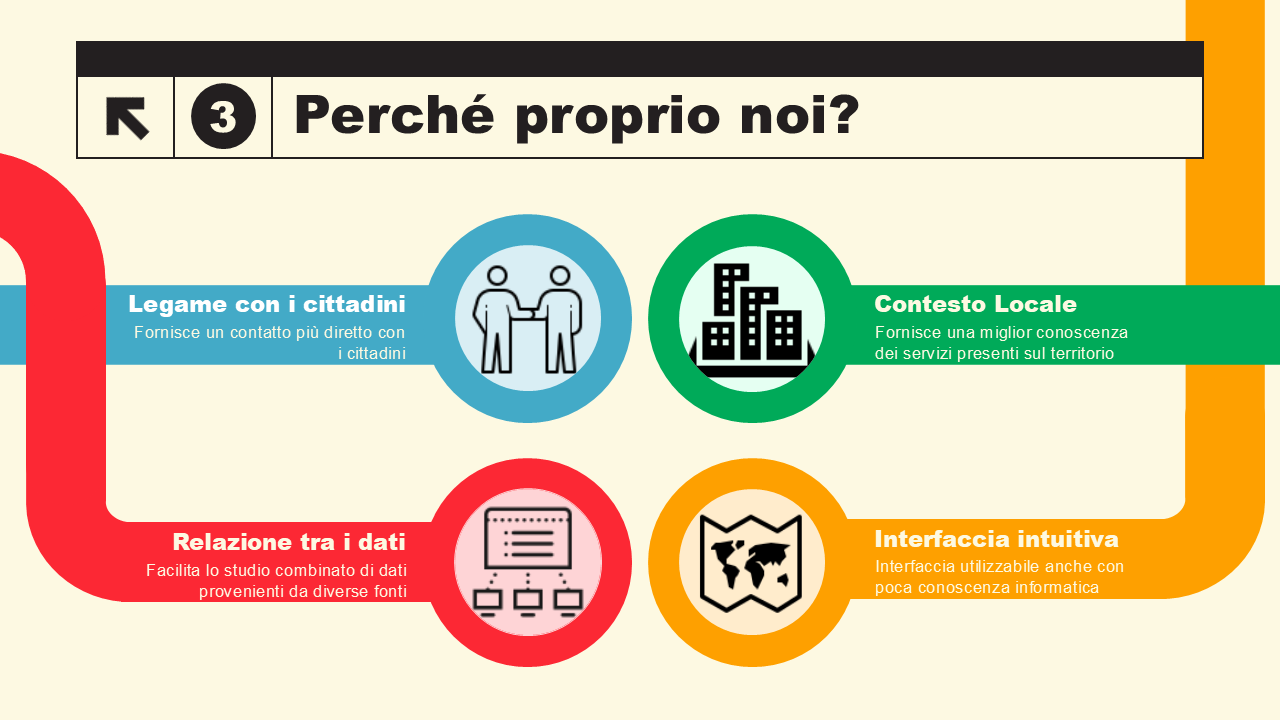
\includegraphics[width=\textwidth]{slides/Diapositiva4.PNG}
        \caption{I vantaggi}
    \end{subfigure}
\end{figure}

\section{I problemi}
    Il progetto mira a risolvere due problemi. Il primo problema riguarda una difficoltà che colpisce l'amministrazione del Comune di Trento, più precisamente la difficoltà stante nel processo di prendere decisioni amministrative efficaci per la città, infatti non raramente accade che una decisione fatta dal Comune non porti al risultato atteso o desiderato. Questo problema nasce dal fatto che, attualmente, il personale del comune non dispone di un modo adeguatamente chiaro, semplice, e organizzato di studiare la mole di dati rilevanti alla situazione della città. Inoltre, i modi esistenti in cui il Comune ottiene un riscontro dai cittadini veri e propri sulla loro soddisfazione con la città sono insufficienti o inaffidabili, rendendo difficile comprendere l'impatto delle decisioni prese in passato. 
    
    Il secondo problema riguarda gli abitanti che si sono trasferiti, sono ancora nel processo di trasferirsi, o sono interessati a trasferirsi, a Trento. Questi nuovi cittadini spesso sono ignari dei servizi a loro disponibili nell'area in cui si trovano, e dunque non sono in grado di usufruirne. Inoltre, non hanno una visione chiara della situazione della città, e dunque non sono in grado di valutare se un particolare quartiere o zona della città sia adatta alle loro esigenze. Questo problema è aggravato dal fatto che i dati sulla città sono spesso dispersi in vari siti web e documenti, e non sono presentati in modo chiaro e comprensibile.

\section{La soluzione}
    L'obbiettivo del progetto è realizzare un'applicazione web che permetterà sia ai cittadini che al personale del Comune di visualizzare in modo intuitivo e comprensibile i dati sui servizi presenti nella città, la grande parte di questi dati è gia stata raccolta, hanno solo bisogno di essere mostrati agli utenti. Oltre a queste informazioni l'applicazione mostrerà anche l'andamento nel tempo del grado di felicità, espresso in percentuale, della popolazione della città e dei singoli quartieri. I dati sulla felicità potranno essere raccolti da tipi di fonti diversi.

    L'applicazione sarà accessibile tramite browser, qualunque utente sarà in grado di vedere dei dati generali sulla città. Il personale del Comune, una volta autenticatosi, avrà accesso ad ulteriori funzionalità per aggiungere, modificare, analizzare, e rimuovere dati dal sistema. Il software sarà conforme alle normative vigenti riguardo la protezione delle informazioni e delle credenziali di accesso degli utenti del Comune.


\section{I vantaggi - sia per il Comune che per i Cittadini}
    \begin{itemize}
        \item \textbf{Legame con i Cittadini:} la possibilità di visualizzare in modo semplice la felicità attuale e passata dei residenti rende possibile al Comune elaborare decisioni indirizzate ai veri bisogni dei cittadini. Permettendo instaurare una relazione di fiducia e collaborazione tra gli abitanti e il Comune.
        \item \textbf{Contesto Locale:} poter visualizzare le caratteristiche di Trento in maniera semplice e chiara permette ai cittadini, sia nuovi che non, di capire in modo più completo l'area intorno a loro e di sentirsi membri di una comunità unita.
        \item \textbf{Relazione tra i Dati:} la creazione di un database delle informazioni sulla città è cruciale per facilitare l'analisi dei dati. Lo schema logico del database permetterà facile l'accesso alla grande quantità e varietà di dati, permettendo di studiare Trento da molti punti di vista diversi. Inoltre, sarà semplice per il personale addetto aggiungere nuovi dati al sistema, assicurando che il l'applicazione continuerà ad essere affidabile e utile per un periodo di tempo esteso.
        \item \textbf{Interfaccia intuitiva:} Presentare le informazioni con un'interfaccia grafica, accessibile anche a utenti sprovvisti di conoscenze informatiche, assicura che l'applicazione sarà utile a una vasta quantità di cittadini, non solo al personale del Comune.
    \end{itemize}
    cd\chapter{Requisiti Funzionali} 
    \section{Requisiti funzionali comuni a tutti gli utenti}
        \begin{rfList}
            \rfItem \textbf{Homepage} Il sistema deve consentire a tutti gli utenti di essere in grado di visualizzare integralmente la mappa del comune di Trento divisa per quartieri non appena si apre la web-app.
            \rfItem \textbf{Interazione con la mappa} Il sistema deve permettere a tutti gli utenti di interagire con la mappa del comune di Trento, in particolare deve essere possibile: ingrandire, rimpicciolire e spostarsi all'interno della mappa tramite il mouse o i pulsanti.
            \rfItem \textbf{Multi lingua} Il sistema deve contenere dei pulsanti a forma di bandiera per cambiare lingua su tutte le pagine del sistema, le lingue che devono essere disponibili nel sistema saranno: italiano, tedesco, e inglese. Quando si preme su uno di questi pulsanti la pagina si ricaricherà nella lingua selezionata e il pulsante della lingua precedentemente selezionata tornerà ad essere disponibile.
            \rfItem \textbf{Accesso dati quartieri} Il sistema deve permettere a tutti gli utenti di selezionare qualunque dei vari quartieri della città. Selezionare un quartiere consentirà all'utente di visualizzare i dati generici (num popolazione, felicità, età media, servizi,\dots) relativi al quartiere selezionato. Inoltre la mappa visualizzata sposterà il focus e si ingrandirà su di questo. Quando un quartiere è selezionato verrà evidenziato, sarà inoltre possibile de-selezionarlo cliccando nuovamente sullo stesso quartiere o cliccando su di un altro quartiere.
            \rfItem \textbf{Accesso dati specifici quartieri} I dati dei vari quartieri saranno visualizzabili in modo più esteso quando viene cliccato su uno specifico dato relativo ad un quartiere (se disponibile). Questo comporterà la visualizzazione di una tabella coi dati estesi relativi al quartiere selezionato, sarà possibile chiudere la tabella cliccando su un pulsante di chiusura. 
        \end{rfList} 
    \section{Requisiti funzionali per tutti gli utenti loggati}
        \begin{rfList}
            \rfItem \textbf{Autenticazione} Il sistema deve permettere a tutti gli utenti loggati di accedere al loro account premendo un tasto di login in altro a destra, il quale renderizzerà gli utenti alla pagina del service provider della provincia di Trento al quale accederanno tramite: il Sistema Pubblico di Identità Digitale (SPID), la Carta Nazionale dei Servizi (CNS), la Carta di Identità Elettronica (CIE) o la carta Provinciale dei Servizi (CPS). Nel caso in cui l'utente non avesse un ruolo abilitato questo verrà reindirizzato alla pagina principale con un messaggio di errore tramite pop-up che informerà dei mancati permessi per accedere al sistema.
            \rfItem \textbf{Cambio icona login} Successivamente al processo di autenticazione per qualsiasi utente loggato verrà sostituita l'icona del login con l'immagine del profilo con il quale si è fatto l'accesso.
        \end{rfList}     
    \section{Requisiti funzionali per i sondaggisti}
        \begin{rfList}
            \rfItem \textbf{Visualizzazione dati sondaggisti} Il sistema deve permettere ai sondaggisti di visualizzare tramite una pagina dedicata, accessibile dalla top-bar dopo aver effettuato il login, una tabella contenente il riassunto dei dati relativi ai sondaggi inseriti da loro stessi con relativo stato di approvazione e se non approvati dei pulsanti per eliminare e/o modificare i dati inseriti. 
            \rfItem \textbf{Accesso come sondaggista} Il sistema successivamente al processo di autenticazione reindirizzerà automaticamente i vari account sondaggisti alla corrispettiva pagina dedicata, così facendo verrà velocizzata e semplificata la procedura d'accesso limitando inoltre le funzionalità fornite ai sondaggisti.
            \rfItem \textbf{Caricamento dati sondaggisti} Il sistema deve permettera ai sondaggisti di aggiungere i dati relativi ai sondaggi eseguiti sul territorio comunale tramite una pagina apposita nella quale verranno inseriti i dati relativi al riepilogo del sondaggio quali il numero di voti cumulato e raggruppati per quartiere. I dati inseriti dai sondaggisti non saranno visibili agli altri utenti e non saranno neanche considerati dal sistema fino a quando non verranno approvati da un utente amministratore. Inoltre sarà possibile caricare i dati mano a mano che il sondaggio viene eseguito da una interfaccia grafica visualizzabile anche da dispositivi mobili.
            \rfItem \textbf{Modifica ed eliminazione dati sondaggisti} Il sistema deve permettere ai sondaggisti di modificare e/o eliminare i dati inseriti da loro stessi andando nella apposita pagina di visualizzazione dei sondaggi inseriti da loro stessi e selezionando il sondaggio che si vuole modificare e/o eliminare. 
        \end{rfList}
    \section{Requisiti funzionali per analisti, circoscrizioni e amministratori}
        \begin{rfList}
            \rfItem \textbf{Modifica Homepage} Per gli utenti: analista, circoscrizione e amministratore, all'interno della Homepage verrà fornita la possibilità di visualizzare una tabella contenente le informazioni più importanti dei vari quartieri (Nome, percentuale di soddisfazione, numero di abitanti) al posto della mappa, sarà inoltre possibile passare dalla visualizzazione della mappa a quella della tabella (o viceversa) attraverso l'utilizzo di un pulsante di selezione.
            \rfItem \textbf{Accesso come analista, circoscrizione o amministratore} Successivamente al processo di autenticazione per gli utenti: analista, circoscrizione e amministratore, verranno reindirizzati alla Homepage modificata con la visualizzazione della città sotto forma di tabella.
        \end{rfList}
    \section{Requisiti funzionali per gli analisti}
        \begin{rfList}
            \rfItem \textbf{Visualizzazione Analisti Database} Il sistema deve permettere agli analisti la possibilità di visualizzare tutti i dati presenti nella base di dati, questo tramite apposite tabelle accessibili. Le tabelle saranno accessibili tramite link resi disponibili nella top-bar dopo che l'utente ha eseguito il login. Per ogni tabella, riguardante i dati, l'analista potrà decidere di filtrare e/o orinare la tabella per uno o più campi, alcuni campi potrebbero non essere filtrabili e/o ordinabili. La tabella visualizzata sarà suddivisa in pagine con un numero di righe predefinite ma modificabile.
            \rfItem \textbf{Visualizzazione Analisti Storico} Il sistema deve permettere agli analisti di visualizzare degli storici riassuntivi tramite grafici dinamici i quali potranno essere filtrati per data di acquisizione del dato visualizzato. Il sistema permetterà inoltre di confrontare due quartieri selezionati dall'analista, mostrando l'andamento del dato selezionato nel tempo, tramite due serie sullo stesso grafico. Il sistema permetterà inoltre di confrontare due dati diversi di uno stesso quartiere, mostrando l'andamento dei due dati nel tempo, tramite due serie sullo stesso grafico. 
        \end{rfList}
    \section{Requisiti funzionali per gli amministratori}
        \begin{rfList}
            \rfItem \textbf{Approvazione-Disapprovazione dati sondaggisti } Il sistema deve permettere agli amministratori di visualizzare tramite una pagina dedicata, accessibile dalla top-bar dopo aver effettuato il login, una tabella contenente il riassunto dei dati relativi ai sondaggi inseriti dai sondaggisti con relativo stato di approvazione, inoltre saranno disponibili dei pulsati per visualizzare nel dettaglio i dati inseriti dai sondaggisti, per approvare i dati inseriti dai sondaggisti, per richiedere la modifica dei dati inseriti dai sondaggisti e per eliminare i dati inseriti dai sondaggisti.
            \rfItem \textbf{Modifica dati statici} Il sistema deve permettere agli amministratori di visualizzare tramite una pagina dedicata, accessibile dalla top-bar dopo aver effettuato il login, una pagina di modifica dei dati relativi ai servizi e/o altro da inserire manualmente nel sistema, dalla stessa pagina sarà possibile aggiungere, modificare e/o eliminare i dati inseriti manualmente.
            \rfItem \textbf{Modifica utenti abilitati} Il sistema deve permettere agli amministratori di visualizzare un riepilogo, tramite pagina dedicata accessibile solo dagli amministratori, degli utenti registrati nel sistema, con la possibilità di visualizzare i dettagli di un utente, di modificare i dati di un utente, di eliminare un utente e di visualizzare i ruoli di un utente, inoltre deve essere possibile assegnare e/o rimuovere un ruolo ad un utente e abilitare un nuovo utente nel sistema. L'abilitazione di un utente nel sistema comporterà l'invio di una mail all'utente notificando l'avvenuta abilitazione.
            \rfItem \textbf{Visualizzazione richieste e risposte} Il sistema deve permettere agli amministratori di visualizzare le richieste inviate dalle circoscrizioni al comune e le risposte inviate tramite una tabella accessibile dalla top-bar dopo aver effettuato il login, nella quale verranno visualizzati l'oggetto della richiesta, il testo della richiesta, se è presente la risposta del comune, l'oggetto della risposta e il testo della risposta.
        \end{rfList}
    \section{Requisiti funzionali per le circoscrizioni}
        \begin{rfList}
            \rfItem \textbf{Aggiunta/modifica dati circoscrizioni} Il sistema deve permettere alle circoscrizioni di aggiungere e/o modificare i dati relativi ai servizi e/o altro da inserire nel sistema, tramite una pagina dedicata accessibile dalla top-bar dopo aver effettuato il login.
            \rfItem \textbf{Invio richiesta al comune} Il sistema deve permettere alle circoscrizioni l'invio di richieste al comune tramite una pagina dedicata accessibile dalla top-bar dopo aver effettuato il login, nella quale verrà inserito l'oggetto della richiesta e il testo della richiesta. Una volta inviata la richiesta verrà inviata una mail al comune e verrà visualizzato un messaggio di conferma dell'invio della richiesta.
            \rfItem \textbf{Visualizzazione richieste e risposte} Il sistema deve permettere alle circoscrizioni di visualizzare le richieste inviate al comune e le risposte ricevute dal comune tramite una tabella, nella quale verranno visualizzati l'oggetto della richiesta, il testo della richiesta, se è presente la risposta del comune, l'oggetto della risposta e il testo della risposta.
        \end{rfList}
    \chapter{Requisiti Non Funzionali} 
\thispagestyle{stdPage}
    \begin{rnfList}
        \rnfItem \textbf{Compatibilità} La web app deve essere compatibile con le seguenti versioni di browser: Chrome 80+, Firefox 80+, Safari 14+, Edge 80+ fornendo a ciascuna una pari esperienza per quanto riguarda il numero delle funzionalità disponibili.
        \rnfItem \textbf{Velocità di risposta} Il sistema deve essere in grado di fornire i dati richiesti all’utente entro 2 secondi dalla loro richiesta, ciò per garantire una esperienza ottimale verso l’utente sia che si tratti di un utente loggato o meno
        \rnfItem \textbf{Multi Utenza} Il sistema deve riuscire a gestire almeno 50 utenti connessi simultaneamente, senza che nessuna funzionalità sia compromessa
        \rnfItem \textbf{Sicurezza Dati} I dati dovranno essere memorizzati in modo sicuro assicurandosi che solo gli addetti ai lavori possano accedere al database direttamente e gli utenti i quali non hanno accesso ad un determinato dato non devono essere in grado di ricavarlo tramite chiamate al backend. Inoltre i dati dovranno essere protetti tramite protocollo \texttt{HTTPS}.
        \rnfItem \textbf{Backup Plan} Il sistema dovrà prevedere un piano di backup dei dati in modo sicuro tramite connessione di trasferimento \texttt{SFTP} su un server locale interno all'edificio (6h/12h/1d) e un backup meno frequente remoto (1d/3d/1w).
        \rnfItem \textbf{Capacità di caricamento} Il sistema deve permettere ai Sondaggisti di caricare anche quantità di dati con unità di misura del Gigabyte in meno di 10 minuti.
        \rnfItem \textbf{Aggiornamento Dati} Il sistema deve permettere di aggiungere/modificare/eliminare i dati regolarmente mantenendo una struttura logica intatta.
        \rnfItem \textbf{Invecchiamento Dati} I dati sulla felicità caricati hanno validità massima di circa 6 mesi al fine di mantenerli attuali.
        \rnfItem \textbf{Facilità d'uso} La parte grafica generale deve essere di facile utilizzo per tutti gli utenti, la parte della web-app disponibile a tutti gli utenti deve essere comprensibile fin dal primo utilizzo ed entro 10 minuti dovrebbe essere chiaro a chiunque come funzioni l'app nella sua interezza.
        \rnfItem \textbf{Facilità di Navigazione} Il sistema farà uso di un design accessibile tramite una navigazione con top-bar accessibile sia da schermi con risoluzione desktop, laptop e tablet.
        \rnfItem \textbf{Multilingua} La lingua selezionata inizialmente deve essere l'italiano, però devono essere disponibili anche la lingua inglese e tedesca.
    \end{rnfList}
    \chapter{Design Front-End}

%capo la mia conoscenza di latex si sta espandendo però probabilmente questo non compila comunque, halp me plz
% ho fatto del mio meglio per preparare un brodo degno di gordon ramsay
% by @Boss314

\section{Pagina Iniziale}

    \label{fig:4.1}
    \begin{figure}[H]
        \center
        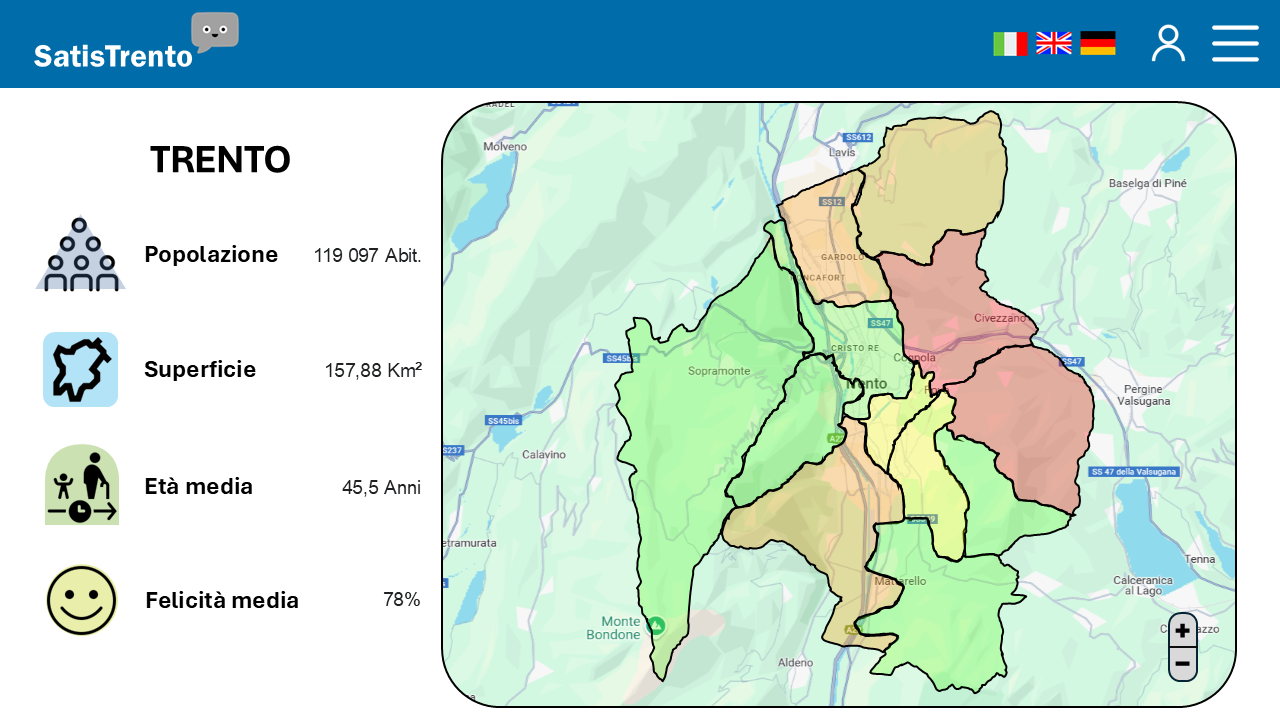
\includegraphics[width=0.6\textwidth]{Interfaccia_grafica/home.PNG}
        \caption{Schermata principale dell'applicazione}
    \end{figure}

    La Figura 4.1 mostra un mockup della pagina principale dell'applicazione, questa schermata sarà visibile a tutti gli utenti, loggati e non loggati.

    \begin{itemize}
        \item \textbf{RF1: Homepage} \begin{itemize}
            \item La homepage dell'applicazione mostra la mappa del Comune di Trento in primo piano, sono visibili anche i confini tra i singoli quartieri della città.
        \end{itemize}
        \item \textbf{RF3: Multi lingua} \begin{itemize} 
                \item L'interfaccia contiene tre pulsanti, ognuno contenente una bandiera corrispondente a una delle lingue supportate dall'applicazione (italiano, inglese, tedesco). Cliccando sui pulsanti cambierà la lingua in cui è presentata l'applicazione.
        \end{itemize}
        \item \textbf{RF6: Autenticazione} \begin{itemize} 
            \item L'interfaccia presenta un pulsante, rappresentato da un'icona a forma di "persona", che permette di iniziare il processo di autenticazione degli utenti. Questo permette agli utenti loggati di accedere al proprio account tramite SPID, CNS, CIE, CPS; come dettato dal requisito.
        \end{itemize}
        \item \textbf{RNF10: Facilità d'uso} \begin{itemize}
                \item La grafica disponibile a tutti gli utenti presenta un design chiaro, usando icone per rendere la navigazione attraverso la web-app il più accessibile e intuitiva possibile.
        \end{itemize}
        \item \textbf{RNF11: Facilità di navigazione} \begin{itemize}
            \item L'interfaccia permette all'utente di navigare facilmente tra le pagine, inoltre è possibile accedere a tutte le funzionalità fornite all'utente selezionato tramite un menù a tendina, che si aprirà cliccando sull'icona ad "hamburger" presente nella parte superiore destra della schermata.
        \end{itemize}
        \item \textbf{RNF12: Multilingua} \begin{itemize} 
            \item All'inizio, l'interfaccia sarà presentata in lingua italiana. Il design include pulsanti, sempre presenti nella parte alta della schermata, per cambiare la lingua in inglese o tedesco.
        \end{itemize}
    \end{itemize}


\newpage
\section{Utente Loggato, Dati in Tabella}

    \begin{figure}[H]
        \center
        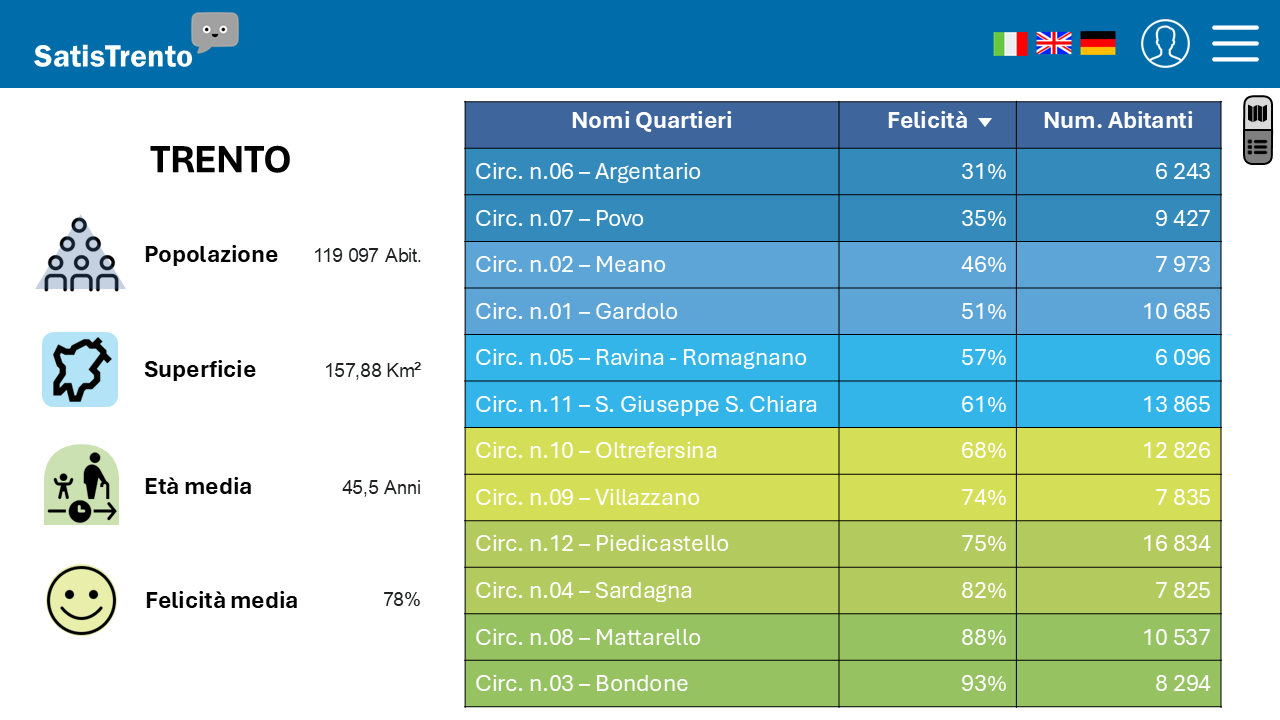
\includegraphics[width=0.6\textwidth]{Interfaccia_grafica/dataDetail.PNG}
        \caption{Dettaglio dati per analisti e amministratori}
    \end{figure}    

    La Figura 4.2 mostra il mockup della schermata di homepage modificata visibile agli utenti di tipo: analista, circoscrizione e amministratore. Questa schermata sarà visibile solo dopo che l'utente ha effettuato l'accesso e sarà visibile solo agli utenti con i privilegi sopra citati.

    \begin{itemize}
        \item \textbf{RF6: Autenticazione} \begin{itemize} 
            \item Inoltre è presente il pulsante per aprire il menù a tendina per permettere all'utente di usufruire delle funzionalità abilitate al proprio utente e di eseguire il logout.
        \end{itemize}
        \item \textbf{RF7: Cambio icona login} \begin{itemize} 
            \item L'icona di login è sostituita da un'icona differente per simboleggiare l'accesso eseguito. Questo permette all'utente di individuare l'account con il quale si ha fatto il login
        \end{itemize}
        \item \textbf{RF12: Modifica Homepage} \begin{itemize}
            \item Sebbene il mockup mostri i dati dell'applicazione in una tabella, questa funzionalità sarà disponibile solo quando l'utente è loggato come analista, amministratore o circoscrizione. Tutti gli utenti non loggati, oppure loggati senza privilegi speciali non avranno la possibilità di visualizzare le diverse zone della città tramite tabella, come mostrato nella \hyperref[fig:4.1]{Figura 4.1}.
            \item Inoltre se si preferisce la visualizzazione tramite "mappa" sarà possibile passare a questa tramite icone presenti nella parte destra della mappa sull'angolo in alto. 
        \end{itemize}
        \item \textbf{RF13: Accesso come analista, circoscrizione o amministratore} \begin{itemize}
            \item Gli utenti: analisti, circoscrizioni e amministratori, dopo aver eseguito l'accesso verranno reindirizzati alla presente interfaccia.
        \end{itemize}
        \item \textbf{RNF10: Facilità d'uso} \begin{itemize}
            \item L'interfaccia è stata progettata per essere il più intuitiva possibile, i dati sono presentati in una tabella la quale potrà essere ordinata e filtrata per facilitare la consultazione. Il tutto tramite pulsanti e icone facilmente riconoscibili. Quali le icone di "mappa" e "tabella" per cambiare la visualizzazione dei dati, oppure le icone di "freccia" per ordinare i dati in base a una colonna specifica.
        \end{itemize}
        \item \textbf{RNF11: Facilità di navigazione} \begin{itemize}
            \item L'interfaccia permette all'utente di navigare facilmente tra le pagine, inoltre è possibile accedere a tutte le funzionalità dell'applicazione tramite il menù a tendina, che si apre cliccando sull'icona standard ad "hamburger" presente nella parte superiore destra della schermata.
            \end{itemize}
    \end{itemize}
\newpage
\section{Selezione di un Quartiere}
    \begin{figure}[H]
        \center
        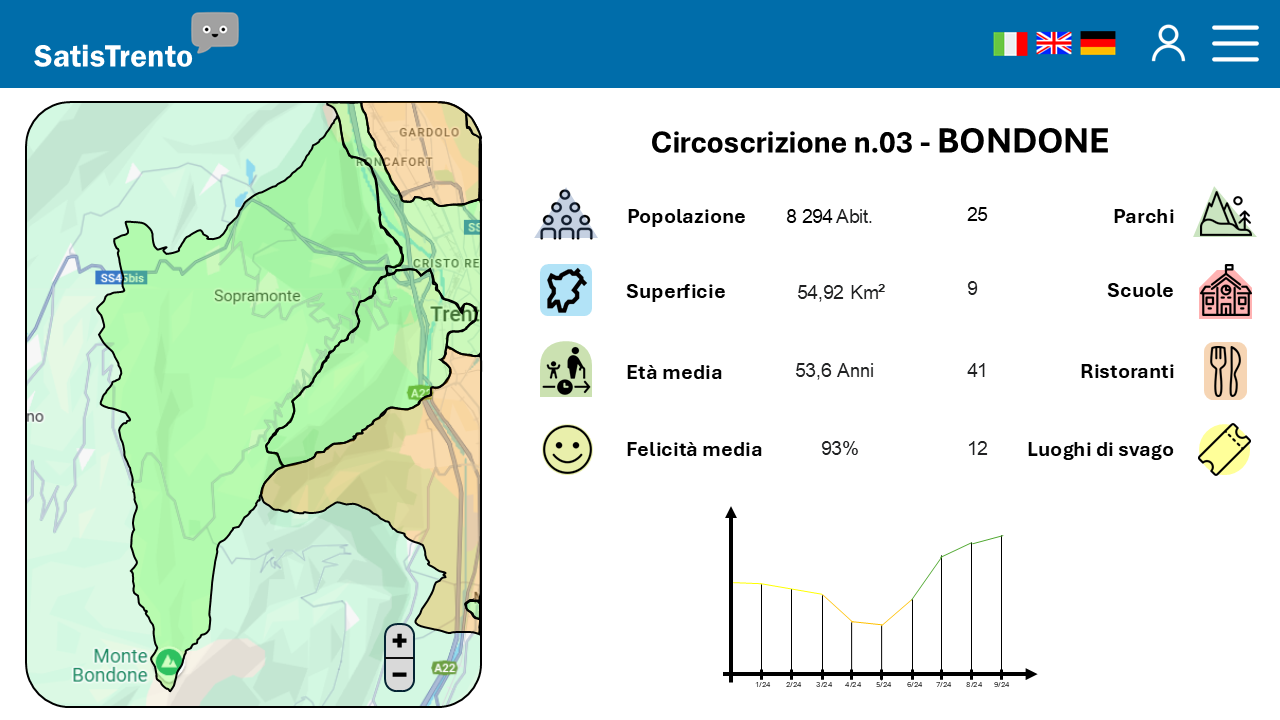
\includegraphics[width=0.6\textwidth]{Interfaccia_grafica/quartiereSelected.PNG}
        \caption{Dettaglio dati per un quartiere selezionato}
    \end{figure}    

    La Figura 4.3 mostra il mockup della schermata visibile dopo che l'utente ha cliccato su uno dei quartieri presenti nella mappa.

    \begin{itemize}
        \item \textbf{RF4: Accesso dati zona selezionata} \begin{itemize}
            \item Ogni zona della città è selezionabile cliccando su di essa utilizzando la mappa. ogni volta che una zona viene selezionata, questa viene ingrandita e mostrata al centro della mappa con le relative informazioni generali  presentate al fianco della mappa. Nel mockup l'interfaccia vengono mostrati solamente i dati generali, visibili dagli utenti non loggati. Ma agli utenti analisti sarà consentito anche osservare i dati più approfonditi raggruppati per tipologia.
        \end{itemize} 
        \item \textbf{RF15: Visualizzazione Analisi Storico} \begin{itemize}
            \item Si noti che è presente un grafico che mostra l'\textbf{andamento nel tempo} del grado di soddisfazione del quartiere selezionato.
            \item Nonostante il grafico e l'analisi nel tempo, sia un requisito specifico per utenti analisti, si è deciso di includere suddetto requisito in quanto questo è un esempio di come l'interfaccia può risultare lato analista.
        \end{itemize}
    \end{itemize}
\section{Caricamento sondaggi e modifica dati}
    \label{fig:4.4}
    \begin{figure}[H]
        \center
        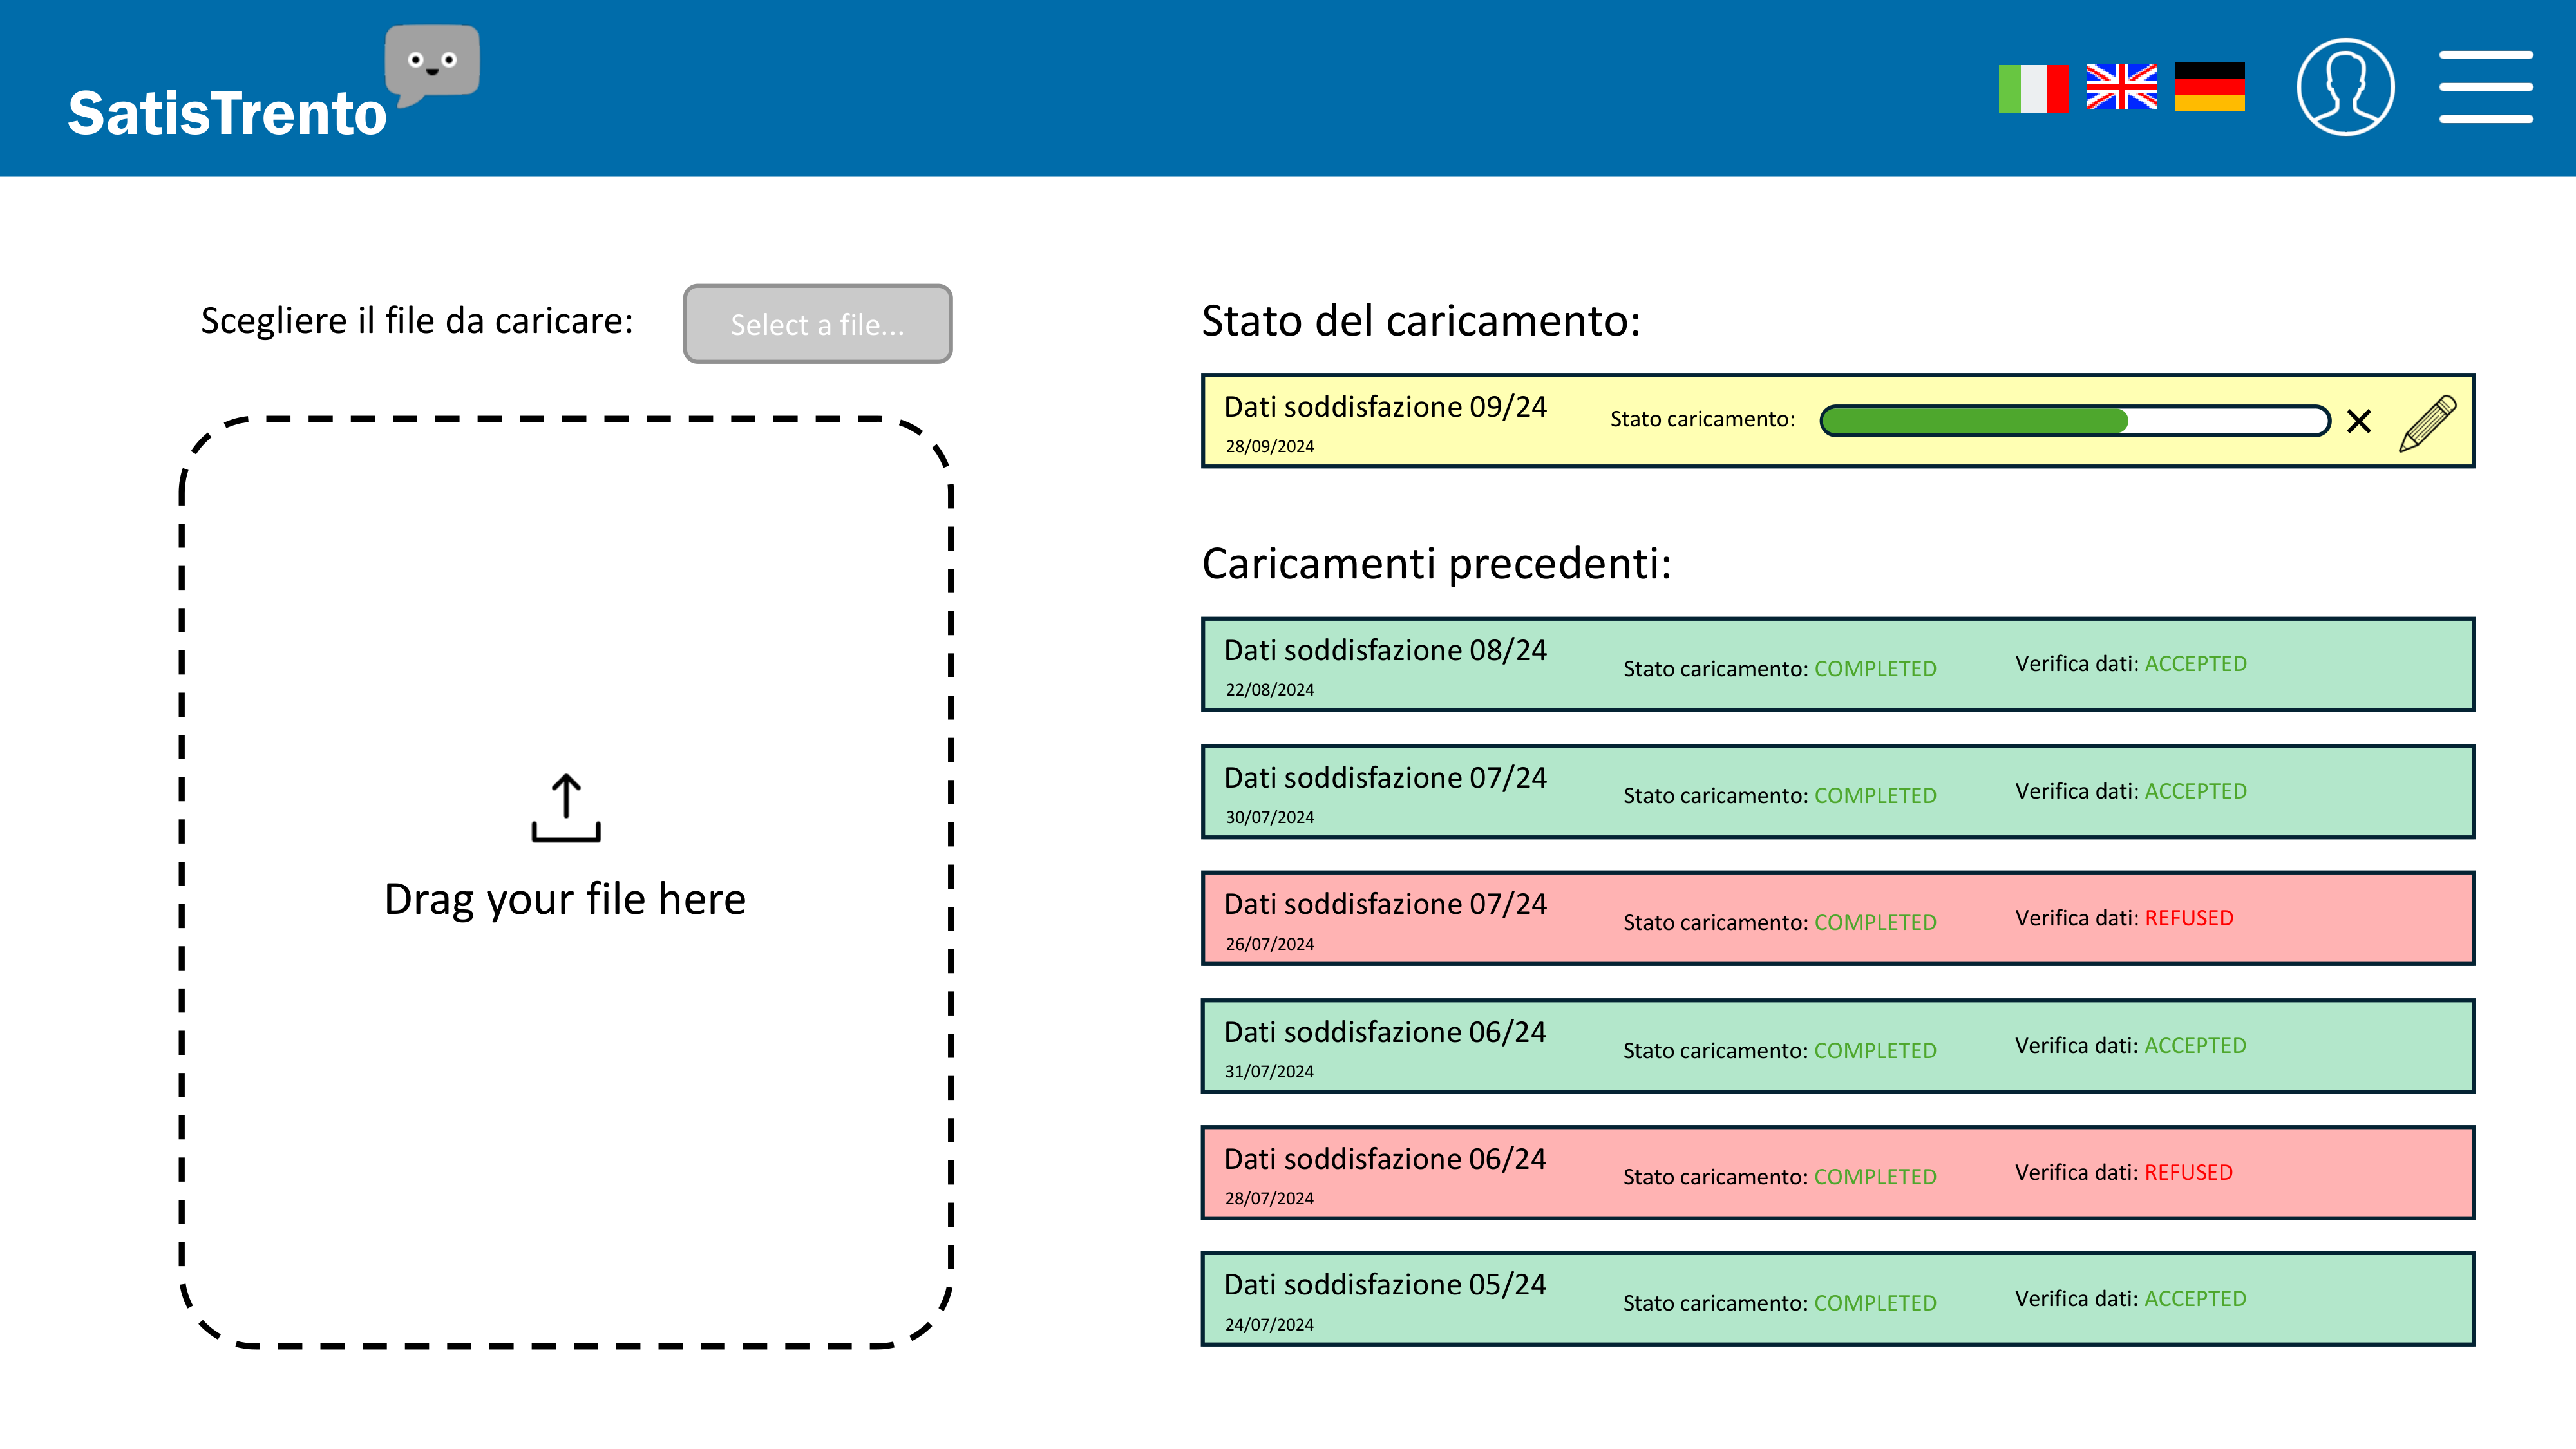
\includegraphics[width=0.6\textwidth]{Interfaccia_grafica/uploadData.PNG}
        \caption{Caricamento dati e visualizzazione elenco}
    \end{figure} 
    La figura 4.4 mostra il mockup della schermata visibile ai sondaggisti e agli amministratori, in cui è possibile caricare i dati sui sondaggi effettuati.\newline
    Il presente layout sarà la base le visualizzazioni lato amministratore per la gestione dei dati e utenti.
    \begin{itemize}
        \item \textbf{RF8: Visualizzazione dati sondaggisti} \begin{itemize}
            \item La seguente pagina permetterà ai sondaggisti di visualizzare i dati caricati da loro stessi, inoltre è presente per ogni sondaggio lo stato di approvazione da parte degli amministratori.
        \end{itemize}
        \item \textbf{RF9: Accesso come sondaggista} \begin{itemize}
            \item Gli utenti: sondaggisti, dopo aver effettuato l'accesso verranno reindirizzati alla presente interfaccia la quale sarà inoltre disponibile solamente a tale tipologia di utente
        \end{itemize}
        \item \textbf{RF10: Creazione nuovi sondaggi} \begin{itemize}
            \item La presente interfaccia permette agli utenti di tipo sondaggista di caricare un file contenente un sondaggio effettuato in precedenza. Inoltre permette di creare un nuovo sondaggio, inserendo i dati generali.
            \item La seguente pagina fungerà da accesso per la modifica e/o eliminazione di dati caricati da sondaggisti non ancora approvati.
        \end{itemize}
        \item \textbf{RF16-17-18-20: Approvazione e disapprovazione sondaggi, modifica dati statici, modifica utenti abilitati} \begin{itemize}
            \item Sebbene la figura rappresenti l'interfaccia delle funzioni per gli utenti sondaggisti, un layout simile può essere usato per l'interfaccia degli utenti amministratori. Tabelle, come quella visibile nella figura, possono essere usate per mostrare i dati statici memorizzati nel sistema e i sondaggi inseriti dai sondaggisti per approvarli o rifiutarli. Un'altra interfaccia simile può permettere agli amministratori di visualizzare e modificare la lista degli utenti loggati e dei loro privilegi.
        \end{itemize} 
        \item \textbf{RNF6: Capacità di caricamento} \begin{itemize}
            \item Questa sarà la principale pagina di caricamento dati sull'applicazione una volta che sull'applicazione saranno caricati i dati di base. In quanto i dati dei sondaggi potrebbero essere pesanti e numerosi, l'interfaccia dovrà essere in grado di gestire il caricamento di grandi quantità di dati in breve tempo.
        \end{itemize}
        \item \textbf{RNF10: Facilità d'uso} \begin{itemize}
            \item Si nota come l'interfaccia è intuitiva e permette all'utente di capire facilmente come caricare i dati e come vedere l'elenco delle informazioni già caricate.
        \end{itemize}
    \end{itemize}

\section{Creazione nuovo sondaggio}

    \begin{figure}[H]
        \center
        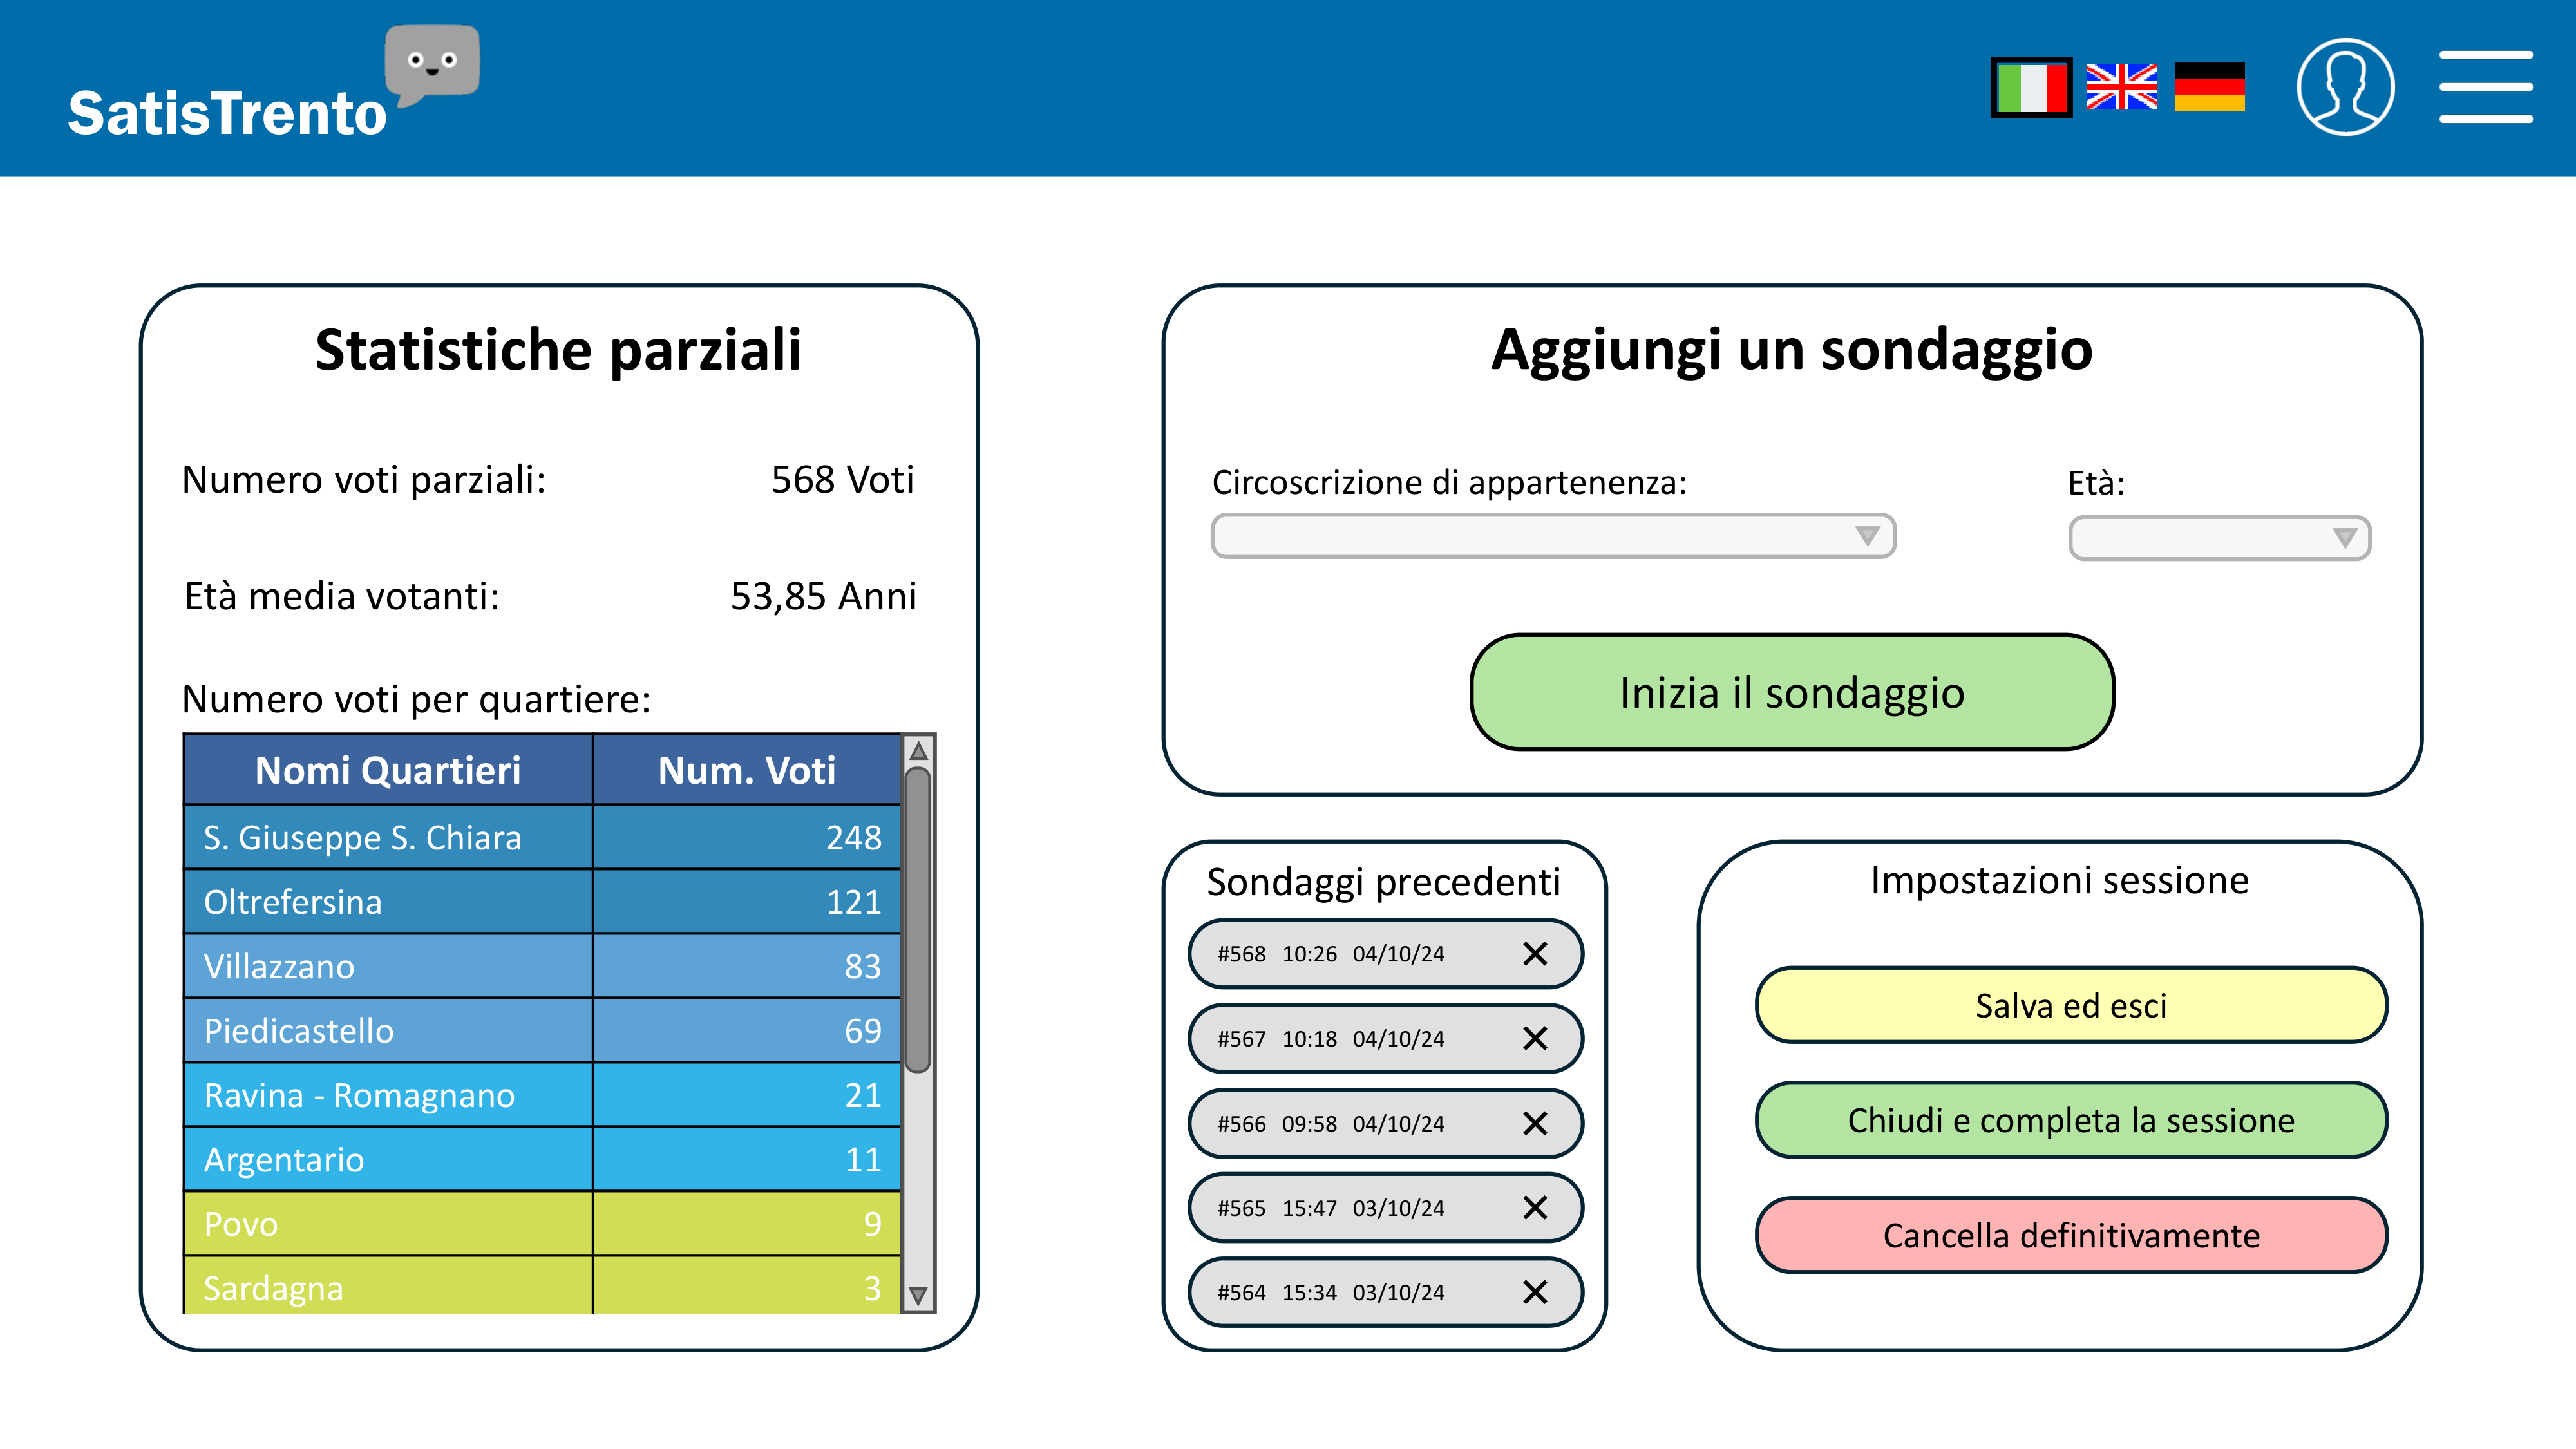
\includegraphics[width=0.6\textwidth]{Interfaccia_grafica/newSurvey.PNG}
        \caption{Schermata della sessione di sondaggio}
    \end{figure}

    La figura 4.5 mostra il mockup della schermata visibile ai sondaggisti durante una sessione di sondaggio. L'interfaccia mostra informazioni sul sondaggio attuale.

    \begin{itemize}
        \item \textbf{RF11: Svolgimento sondaggi} \begin{itemize}
            \item L'interfaccia permette ai sondaggisti di aggiungere nuovi voti al sondaggio attuale, selezionando circoscrizione di appartenenza e età.
            \item Da questa interfaccia è anche possibile: visualizzare i dati raccolti fino a quel momento, chiudere la sessione di sondaggio e inviare i dati per la revisione, sospendere la sessione per continuare in un secondo momento oppure eliminare tutti i dati raccolti fino a quel momento.
            \item Infine sempre dalla seguente interfaccia è possibile vedere un elenco dei voti raccolti fino a quel momento, con la possibilità di eliminare i voti singolarmente.
        \end{itemize}
    \end{itemize}
    
    % \afterpage{\blankpage} % Uncomment this line if to print as a booklet
\end{document}